\qcontributor{Alex Devonport}

\section{Interpolation}

During the control theory module of the course, we encountered the notion of \emph{sampling}; that is, taking a continuous time signal $y(t)$ and converting into a discrete-time signal $y_d(k)$ by taking \emph{samples} at a given time step $\Delta$. Expressed in symbols, we would say $y_d(k)=y(\Delta k)$.
The notion of doing the opposite (that is, converting a discrete-time signal $y_d(k)$ into a continuous-time signal $y(t)$ in such a way that $y(k\Delta)=y_d(k)$) is called \emph{interpolation}.

Interpolation is an important -- and indeed necessary -- part of any discrete-time system that interacts with the real world, since the real world is always in continuous-time.
In other words, interpolation allows for an \emph{interface} between discrete information and the continuous world.
In its role as an interface, we have actually already met interpolation, as we used it implicitly during the control theory module.
Recall that for a sampled discrete-time system, applying the discrete-time control $u(k)=y$ actually means that we apply the constant continuous-time input $u(t)=y$ over the interval $k\Delta\le t \le (k+1)\Delta$ to the continuous-time system.
This means that $u(t)$ is an \emph{interpolation} of $u(k)$ -- specifically a \emph{zero-order hold} interpolation, as you'll see below.

Another important use of interpolation is in \emph{reconstruction} of a continuous-time signal that was converted to a discrete-time system previously.
Consider a continuous-time audio signal, for example.
In order to be stored in digital memory, or to be transmitted digitally, this signal must be sampled into discrete-time.
However, the human ear hears in continuous-time. 
So when the time comes to listen to the audio signal, the signal must be interpolated \emph{back} into continuous-time. 
In other words, the original signal must be reconstructed.
An interesting and practical question is whether or not we can ever reconstruct the signal \emph{perfectly} from the samples; we haven't shown you the tools needed to answer that question yet, but you'll want to keep it in mind.

The essential strategy for interpolating a signal is to express the interpolation as a weighted sum of some chosen continuous-time functions $\phi_i(t)$; that is, to write
\begin{equation*}
 y(t) = \sum_i \alpha_i \phi_i(t),
\end{equation*}
where the $\alpha_i$ weights on functions $\phi_i(t)$ are determined by the specific discrete-time samples $y_d(k)$ in question. 
From this general starting point, two specific methods emerge: the method of \emph{interpolation by basis functions}, and the method of \emph{interpolation by global polynomials}.

\section{Interpolation by Basis Functions}

In this method, we construct the interpolation rather directly, as
\begin{equation*}
 y(t) = \sum_{k=0}^{N-1} y_d(k) \phi(t-k\Delta),
\end{equation*}
where $\phi(t)$ is a \emph{basis function}
\footnote{Based on the similarity of the name, you probably suspect that basis functions are related to the basis of a vector space in some way.
This is actually correct, in a way, but an exploration of this relationship is sadly out of scope.}
of our choosing. 
The basis function $\phi$ may be any function we like that has the following two properties:
\begin{itemize}
 \item $\phi(0)=1$;
 \item $\phi(k\Delta)=0$ for all $k\ne 0$.
\end{itemize}
That is, the function is $1$ when $k=0$ and $0$ at all other $k$ multiples of $\Delta$.
These two properties ensure that the $y(t)$ we constructed in the summation above satisfies $y(k\delta)=y_d(k)$.

This method gives us lots of interpolation schemes. 
For every new basis function we come up with, we get a new interpolation scheme. 
Several common interpolation schemes can be written in terms of basis functions.
For example, zero-order hold (ZOH) interpolation can be expressed using a box-shaped basis function in this way:

\begin{center}
\raisebox{-.5\height}{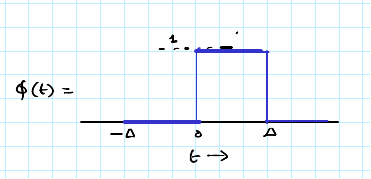
\includegraphics[width=0.45\textwidth]{\bank/interpolation/\bank/interpolation/figs/phibox}}
{\Huge $\Longrightarrow$}
\raisebox{-.5\height}{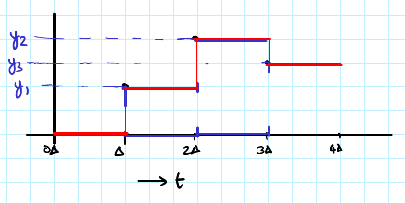
\includegraphics[width=0.45\textwidth]{\bank/interpolation/figs/zoh-interp}}
\end{center}

Similarly, piecewise linear (PWL) interpolation can be expressed using a triangle-shaped basis function:

\begin{center}
\raisebox{-.5\height}{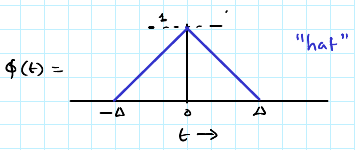
\includegraphics[width=0.45\textwidth]{\bank/interpolation/figs/phihat}}
{\Huge $\Longrightarrow$}
\raisebox{-.5\height}{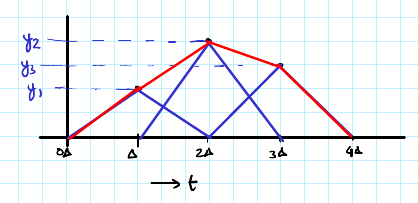
\includegraphics[width=0.45\textwidth]{\bank/interpolation/figs/pwl-interp}}
\end{center}

Another useful basis function is the \emph{sinc} function $\text{sinc}(x)= \frac{\sin(\pi x)}{\pi x}$, where we take $\phi(t)=\text{sinc}(t/\Delta)$.
The sinc function is differentiable and \emph{band-limited}, the importance of which will become clear in the DFT module.

\begin{center}
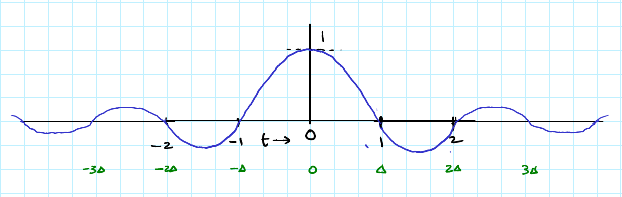
\includegraphics[width=0.75\textwidth]{\bank/interpolation/figs/sinc}
\end{center}


\section{Interpolation by Global Polynomials}

Another method of interpolation is to find a polynomial that passes through the discrete-time data. 
In other words, we can construct $y(t)$ as
\begin{equation*}
 y(t) = \sum_{i=0}^{N-1} a_i t^i,
\end{equation*}
where the $a_i$ are chosen in such a way that $y(k\Delta)=y_d(k)$. 
That is, we are summing polynomials $t^i$ weighted by $a_i$ to reconstruct the continuous-time signal.
Notice that, since $t^i$ do not satisfy the basis function properties, this method is distinct from the basis function method.

How can we choose $a_i$ so that $y(t)$ is a valid interpolation? Since we require that $y(k\Delta)=y_d(k)$ for $0\le k \le N-1$, it turns out that we have a system of linear equations for $a_i$, namely
\begin{align*}
y_d(0) &= a_0\\
y_d(1) &= a_0 + a_1 \Delta + a_2 \Delta^2 + \dotso + a_{N-1} \Delta^{N-1}\\
y_d(2) &= a_0 + a_1 (2\Delta) + a_2 (2\Delta)^2 + \dotso + a_{N-1} (k\Delta)^{N-1}\\
&\vdots\\
y_d(N-1) &= a_0 + a_1 (N-1)\Delta + a_2 ((N-1)\Delta)^2 + \dotso + a_{N-1} ((N-1)\Delta)^{N-1}.\\
\end{align*}
Since we have $N$ equations and $N$ unknowns, we can try to solve for the $a_i$ using these equations. We write the above system of equations in matrix form as
\begin{equation*}
\begin{bmatrix}
y_d(0) \\ y_d(1) \\ y_d(2) \\ \vdots \\ y_d(N-1)
\end{bmatrix}=
\begin{bmatrix}
1 & 0 & 0 & \hdots & 0\\
1 & \Delta & (\Delta)^2 & \hdots & \Delta^{N-1}\\
1 & 2\Delta & (2\Delta)^2 & \hdots & (2\Delta)^{N-1}\\
\vdots & \vdots & \vdots & \vdots & \vdots\\
1 & (N-1)\Delta & ((N-1)\Delta)^2 & \hdots & ((N-1)\Delta)^{N-1}\\
\end{bmatrix}
\begin{bmatrix}
a_1 \\ a_2 \\ \vdots \\ a_{N-1}
\end{bmatrix},
\end{equation*}
which we will write as $\vec{y} = V \vec{a}$ for brevity. Now we can solve for $\vec a$ to get the interpolating polynomial, as long as the matrix $V$ is invertible. 

It turns out that the determinant of this matrix is
\begin{equation*}
 \det(V) = \prod_{0\le i \le j \le N-1} (j\Delta-i\Delta) = (\Delta)(2\Delta)\dotso((N-1)\Delta)
 =(N-1)!\Delta \ne 0
\end{equation*}
due to the \emph{Vandermonde structure} of the matrix.
Since $V$ always has a nonzero determinant, we know that $\vec{y}=V\vec{a}$ always has a unique solution that we can find. Interestingly, it also means that the polynomial interpolation of a discrete-time signal is unique.
